%---------------------------------
\vspace{-0.3em}
\section{Experimental Results}
\label{sec:result}
%---------------------------------

%---------------------------------
\subsection{Experimental settings}
\label{subsec:experiment_setting}
%---------------------------------

\paragraph{Implementation Details.} 
We adopt the VideoCrafter~\cite{chen2023videocrafter} as our base T2V model, which shares the same spatial weights with Stable Diffusion 2.1. We first train the style modulation on image dataset, i.e. WikiArt~\cite{phillips2011wiki} and Laion-Aesthetics-6.5+~\cite{schuhmann2022laion} for 40k steps with a batch size of 32 per GPU.  In the second stage, we froze the style modulation part and only train temporal blocks of VideoCrafter, we jointly train image datasets and video datasets(subset of WebVid-10M~\cite{bain2021frozen}) for 20k steps with a batch size of 1 on video data and 16 on image data, sampling image batches with a ratio of 20\%. The training process is performed on 8 A100 GPUs and can be completed within 3 days. Furthermore, to ensure a fair comparison with some SDXL-based models~\cite{ye2023ipadapter, hertz2023style} on stylized image generation, we also trained the first stage of StyleCrafter on SDXL~\cite{podell2023sdxl}. 
%The overall training process takes about 5 days on 8$\times$V100.

% We train the style adapter on xx for xx epoches, with xx frozen and only train xxxx. In the second stage, xxx. We use xx optimizer and learning rate of xxxx. Also, training dataset.  \TODO{complete this part}

\paragraph{Testing Datasets.}
\label{sec:test_dataset}
To evaluate the effectiveness and generalizability of our method, we construct testsets comprising content prompts and style references. For content prompts, we use GPT-4~\cite{openai2023gpt4v} to generate recognizable textual descriptions from four meta-categories~(human, animal, object, and landscape). We manually filter out low-quality prompts, retaining 20 image prompts and 12 video prompts. For style references, we collect 20 stylized images and 8 sets of style images with multi-reference~(each contains 5 to 7 images in similar styles) from the Internet. In total, the test set contains 400 pairs for stylized image generation, and 300 pairs for stylized video generation (240 single-reference pairs and 60 multi-reference pairs). Details are available in the supplementary materials.

% 1. Content Prompt(generated from GPT4)
% 2. Style Image(selected from internet)
% 3. Content Image(generated from SD, for some style transfer method)
% 4. Style Prompt(generated from GPT4-v, for sd and video-crafter)

\paragraph{Evaluation Metrics.}
\label{sec:eval_metrics}
Following previous practice~\cite{zhang2023inversion, sohn2023styledrop, wang2023styleadapter}, we employ CLIP-based~\cite{radford2021learning} scores and DINO-based~\cite{caron2021emerging} scores to measure the text alignment and style conformity. Following EvalCrafter~\cite{liu2023evalcrafter}, we measure the temporal consistency of video generation by (i) calculating clip scores between contiguous frames and (ii) calculating the warping error on every two frames with estimated optical flow. 
Note that these metrics are not perfect. For example, one can easily achieve a close-to-1 style score by entirely replicating the style reference. Similarly, stylized results may yield inferior text scores compared to realistic results, even though both accurately represent the content descriptions. We recommend a comprehensive consideration of both CLIP-based text scores and style scores, rather than relying solely on a single metric.

\paragraph{User Preference Study.}
In addition to quantitative analysis, we conducted a user study to make comparisons among our method, VideoCrafter, Gen-2, and AnimateDiff in the context of single-reference and multi-reference stylized video generation. Users are instructed to select their preferred option based on style conformity, temporal quality, and all options fulfill text alignment for each comparison pair. We randomly chose 15 single-reference pairs and 10 multi-reference pairs, collecting 1125 votes from 15 users. 
Further details can be found in the supplementary materials.

%
\begin{table*}[!t]
\centering
%\setlength{\tabcolsep}{3.0pt}
% \renewcommand\arraystretch{1.5}
\caption{Quantitative comparison on single-reference style-guided T2I generation. We conduct evaluation on a test set of 400 pairs. \textbf{Bold}: Best. }
\label{tab:img_quan_clip}
\vspace{-1em}
\resizebox{0.93\linewidth}{!}{
  \begin{tabular}{ccccccccc} % {@{}lc@{}}
    \toprule
     \multirow{2}{*}{Method} & \multicolumn{4}{c}{\textbf{Stable Diffusion 2.1 based}} & \multicolumn{4}{c}{\textbf{SDXL based}} \\
    \cmidrule(lr){2-5}\cmidrule(lr){6-9}
     & Dreambooth & InST & SD* & Ours & IP-Adapter-Plus & Style-Aligned & SDXL* & Ours(SDXL)  \\
    \midrule
    \texttt{CLIP-Text} $\uparrow$ & \textbf{0.3047}  & 0.3004 & 0.2766 & 0.3028 & 0.2768 & 0.2254 & 0.2835 & \textbf{0.2918} \\
    \texttt{CLIP-Style} $\uparrow$ & 0.3459 & 0.3708 & 0.4183 & \textbf{0.4836} & 0.5182 & 0.5515 & 0.4348 & \textbf{0.5615} \\
    \texttt{DINO-Style} $\uparrow$ & 0.2278 & 0.2587 & 0.2890 & \textbf{0.3652} & 0.4367 & 0.4395 & 0.2912 & \textbf{0.4514} \\
    \bottomrule
  \end{tabular}
}
\end{table*}



%---------------------------------
\subsection{Style-Guided Text-to-Image Generation}
\label{subsec:image_eval}
%---------------------------------

As mentioned in Sec.~\ref{subsec:style_modulation} and Sec.~\ref{subsec:experiment_setting}, our proposed method also supports to generate stylized images~(using model before temporal finetuning). We are interested to evaluate our method against state-of-the-art style-guided T2I synthesis methods, which are better-established than video counterparts. The competitors include optimization-based methods like DreamBooth~\cite{dreambooth}, inversion-based methods such as InST~\cite{zhang2023inversion} and Style-Aligned~\cite{hertz2023style}, and adapter-based methods like IP-Adapter-Plus~\cite{ye2023ipadapter}. Besides, we consider two unique competitors: SD*~\cite{ldm} and SDXL*~\cite{sdxl}~(text-to-image models equipped with GPT-4V~\cite{openai2023gpt4v}, where GPT-4V generates textual descriptions about the reference's style and merges them with content prompts as input for models). This comparison aims to validate the advantages of employing image conditions to enhance stylized generation instead of relying solely on text conditions.
Implementation details of competitors are available in supplementary materials.
% For each style, DreamBooth and CustomDiffusion are optimized with the provided single reference image to learn the customized concept of style.
%This setting may degrade their performance (because they usually requires 5~20 images to learn a concept) but it is fair comparison since all the methods are only provided with a single style image.

The quantitative comparison is tabulated in Table~\ref{tab:img_quan_clip}. 
% Although our method achieved the best performance on both metrics, we would like to emphasise that clip-based metrics are imperfect.As discussed in Sec.~\ref{sec:eval_metrics}, the CLIP-Text is measured by the similarity between content text embedding and stylized image embedding, the stylistic appearance actually hinders the metric in some extent, which makes those methods with weak stylistic effects (i.e. close to photorealism) achieve superior scores. 
Results reveal that Dreambooth~\cite{dreambooth} and InST~\cite{zhang2023inversion} struggle to accurately capture the style from various style references and exhibit low style conformity. SD*~\cite{ldm} and SDXL~\cite{sdxl} demonstrate good stylistic ability but still fail to reproduce the style of the reference image, possibly because of the text’s inherent clumsiness in expressing specific styles despite utilizing the powerful GPT4V for visual style understanding. IP-Adapter~\cite{ye2023ipadapter} and style-aligned~\cite{hertz2023style} generate aesthetically pleasing images, while their style-content decoupled learning is not perfect and exhibits limited control over content.
In contrast, our method efficiently generates high-quality stylized images that align with the content of the texts and resemble the style of the reference image. Our method demonstrates stable stylized generation capabilities when dealing with various types of prompts.


%---------------------------------
\subsection{Style-Guided Text-to-Video Generation}
\label{subsec:video_eval}
%---------------------------------

\begin{figure*}[t!]
    \centering
    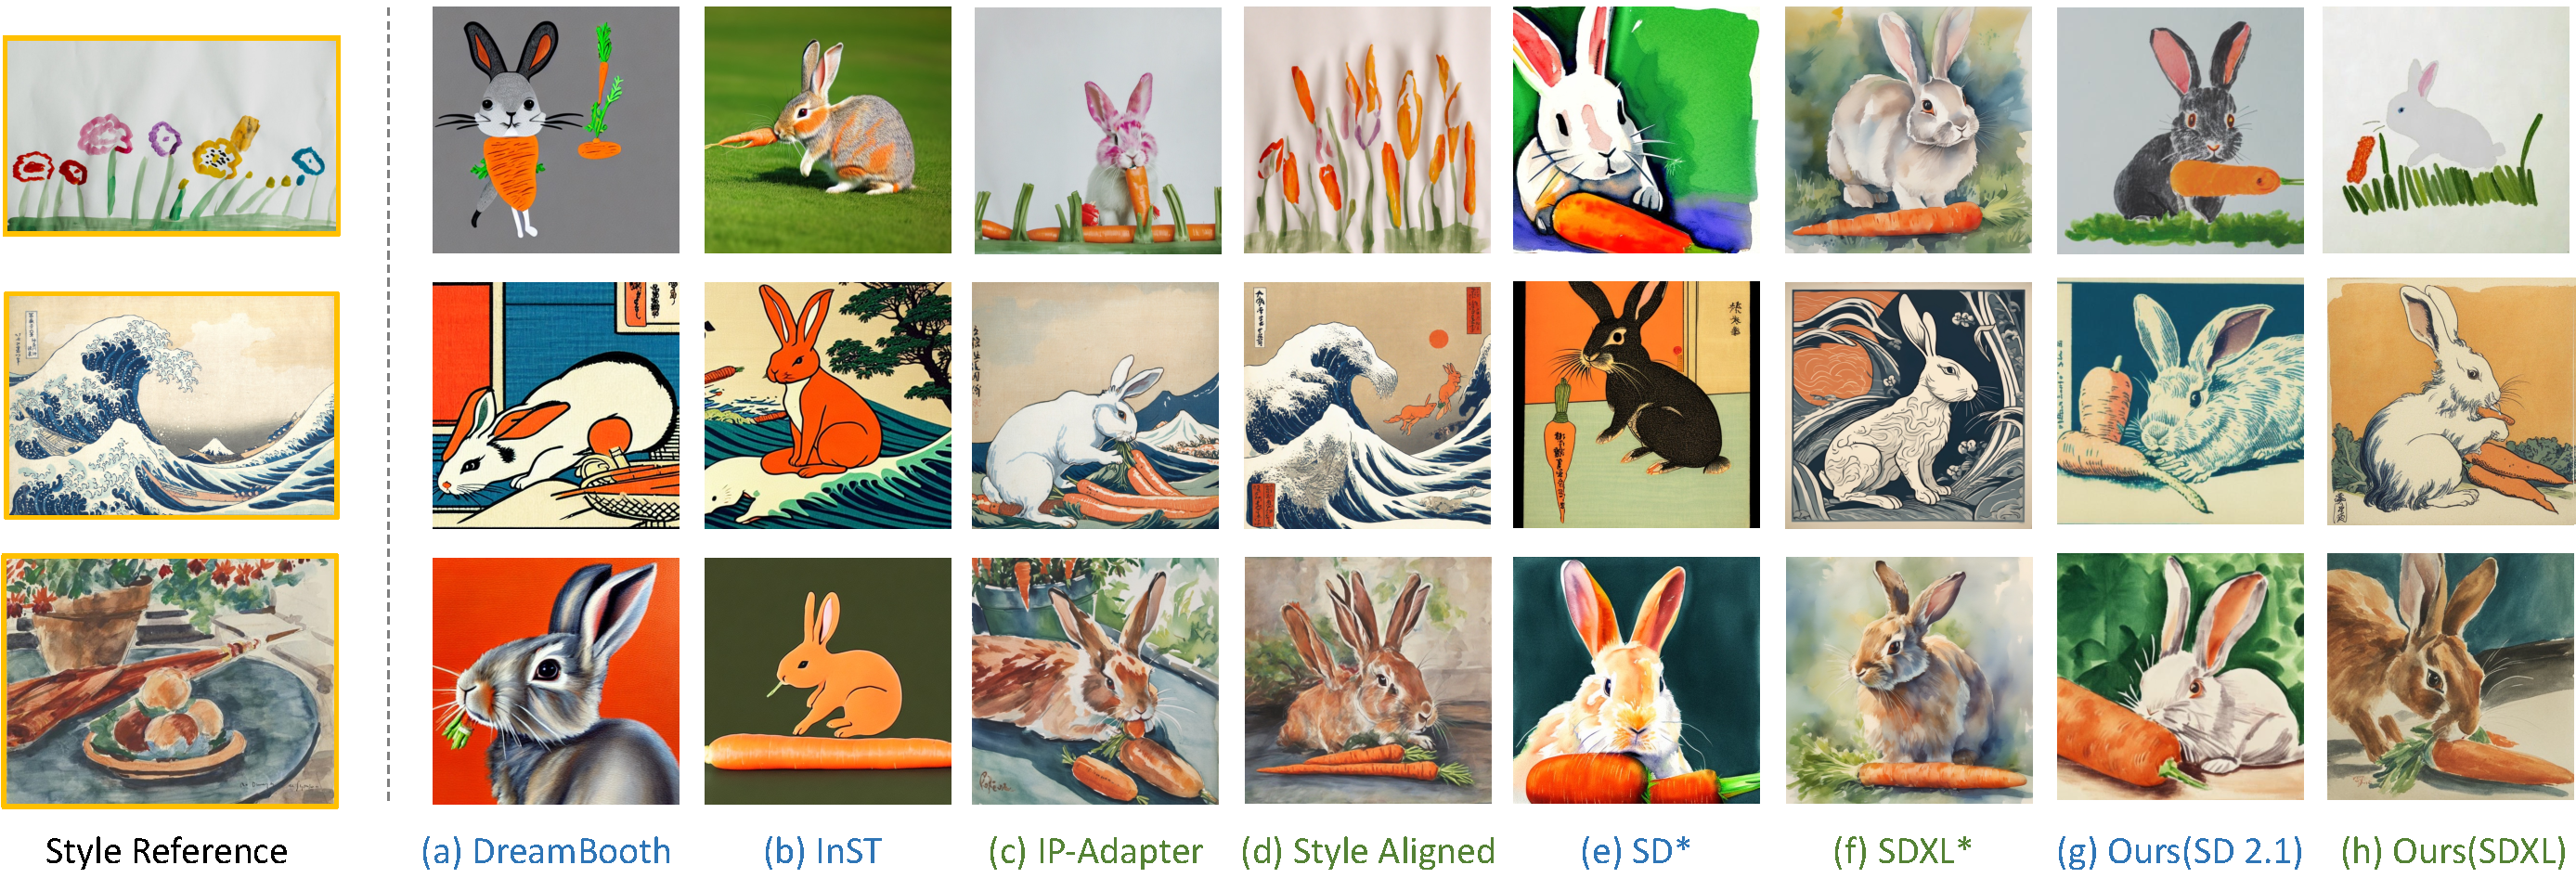
\includegraphics[width=0.87\linewidth]{figures/comp_image.pdf}
    \vspace{-1em}
    % \vspace{-2em}
    \caption{Visual comparison on style-guided T2I generation. \textcolor[RGB]{46, 117, 182}{Blue}: methods based on SD 2.1. \textcolor[RGB]{84, 130, 53}{Green}: based on SDXL. Prompt: A rabbit nibbling on a carrot.} 
    \label{fig:result_img}
    \vspace{-1em}
\end{figure*}
%
\begin{figure*}[!h]
    \centering
    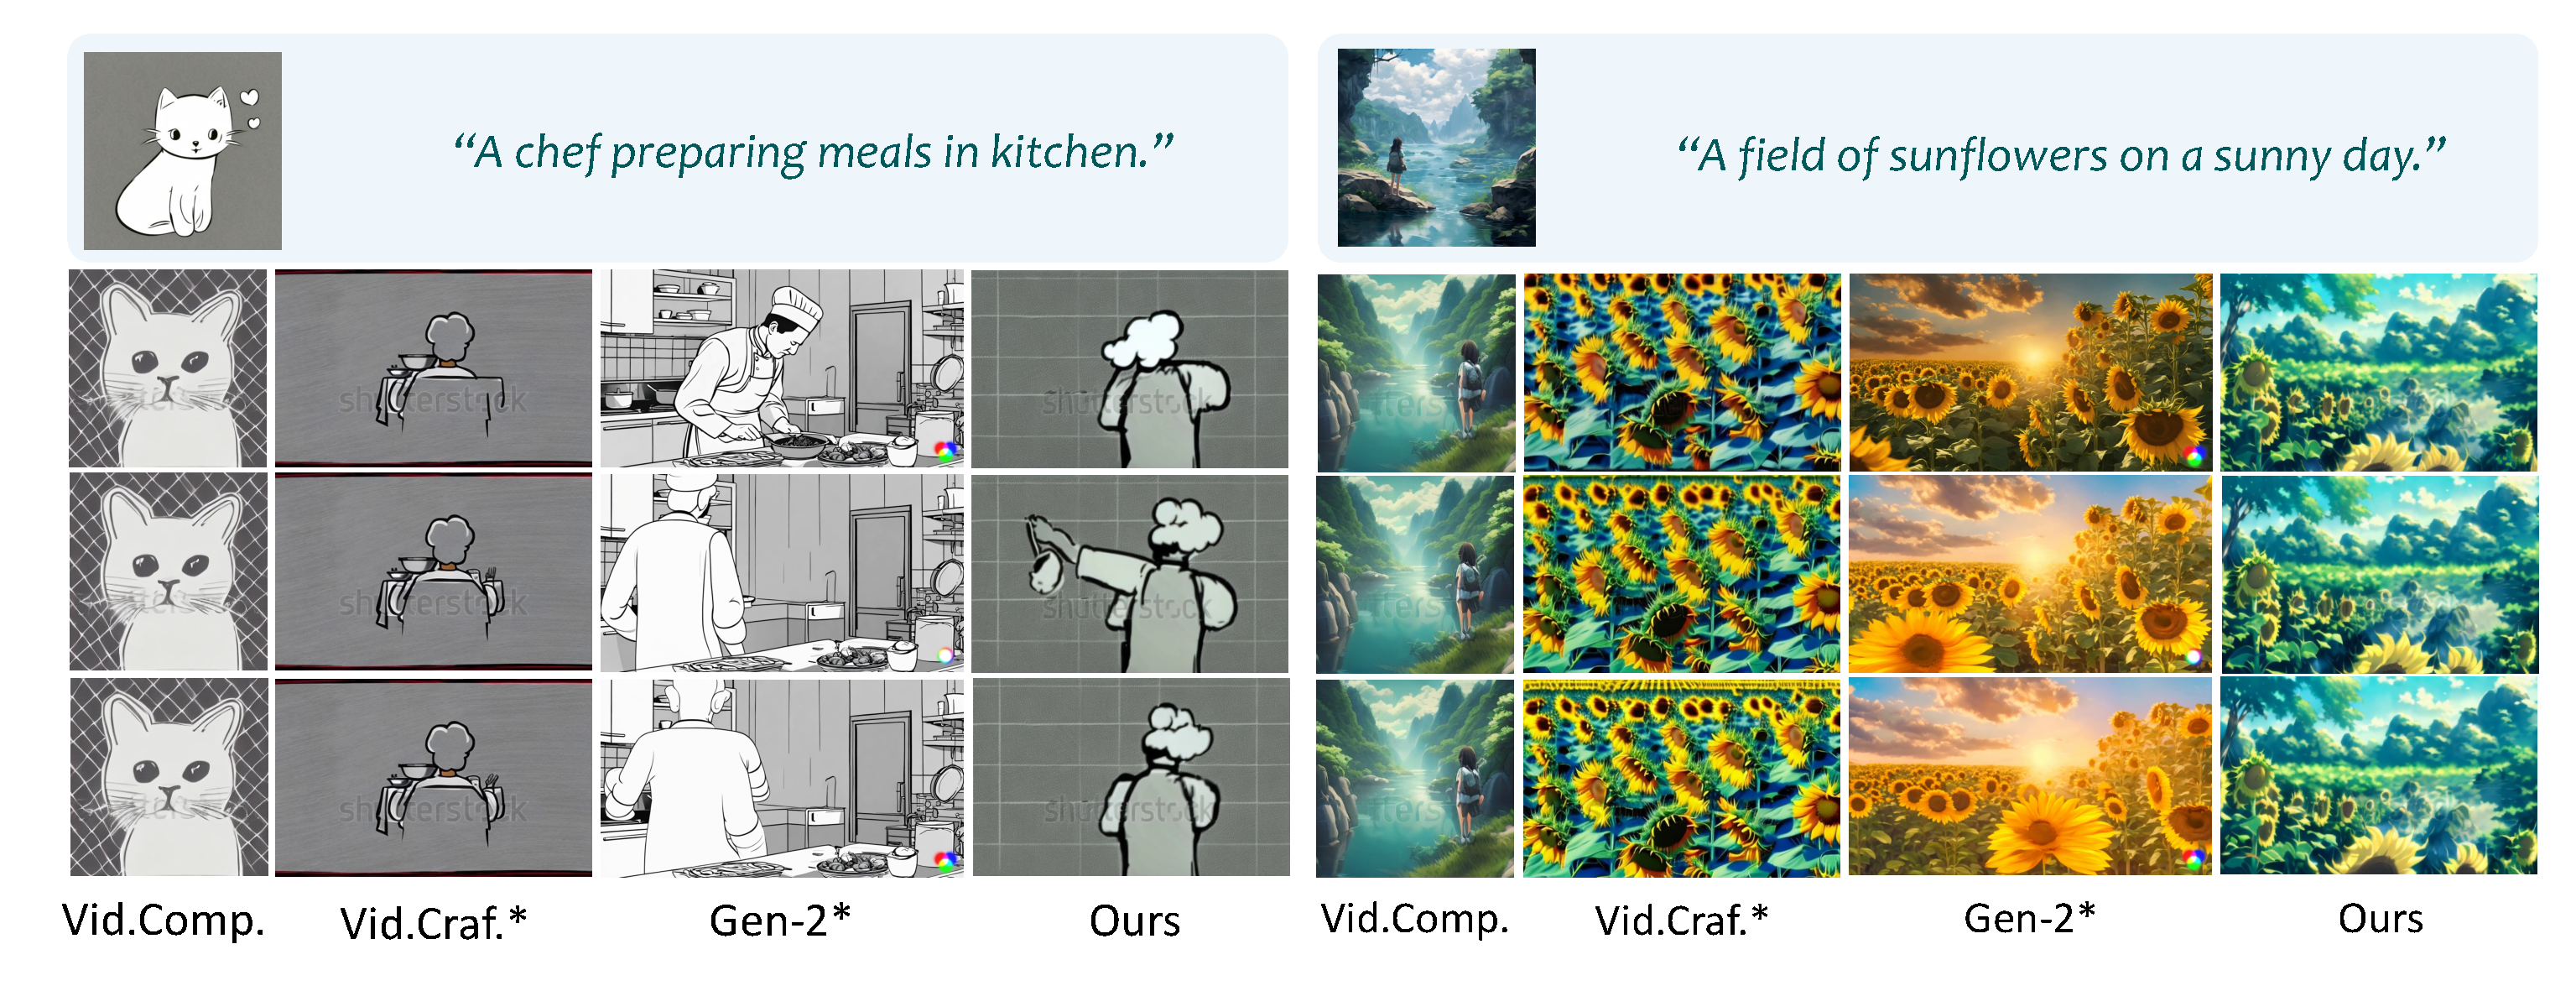
\includegraphics[width=0.9\linewidth]{figures/comp_video.pdf}\vspace{-1.5em}
    \caption{Visual comparison of single-reference guided T2V generation. Vid.Comp.: VideoComposer, Vid.Craf.: VideoCrafter
    %Our approach accurately captures the style of the reference image and generates videos that satisfy both text alignment and style conformity.
    } 
    \label{fig:result_video}
    \vspace{-1em}
\end{figure*}
%
\begin{figure*}[!h]
    \centering
    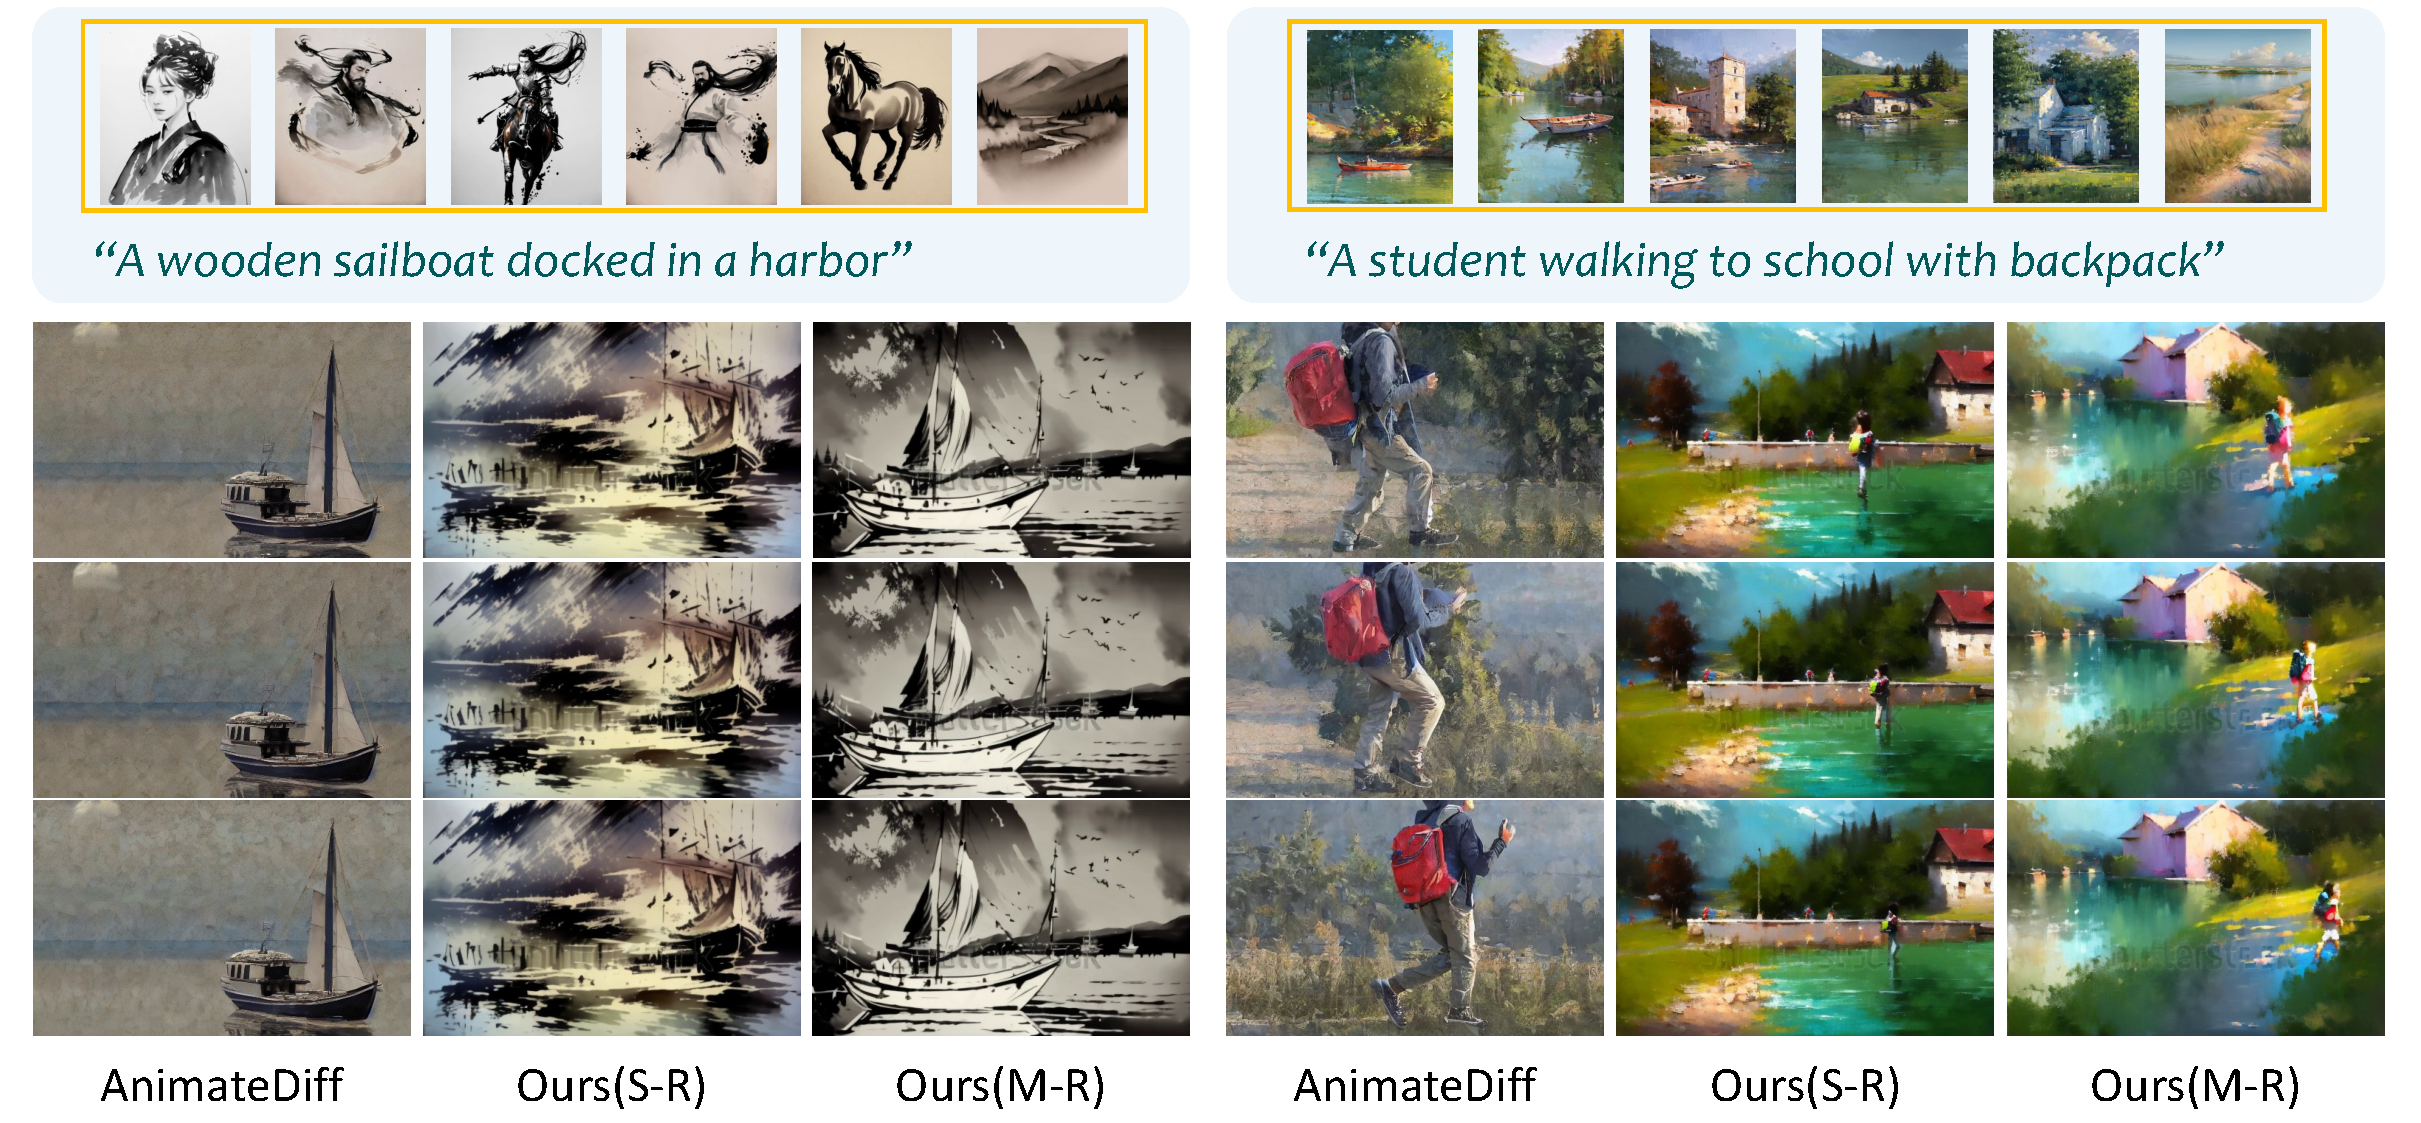
\includegraphics[width=0.87\linewidth]{figures/comp_video2.pdf}
    \vspace{-1em}
    \caption{Qualitative comparison of multi-reference style-guided T2V generation. S-R: Single-Reference, M-R: Multi-Reference
    %AnimateDiff tends to generate close-to-reamlism results despite the style references are typical artistic styles. In contrast, our approach performs better in text alignment, style conformity and temporal consistency.
    } 
    \vspace{-1em}
    \label{fig:result_multi_ref}
\end{figure*}



\begin{table}[!t]
\centering
\caption{Quantitative comparison of style-guided T2V generation. Top 3 rows: single-reference based gudiance. Bottom 3 rows: multi-reference based guidance. S-R: Single-Refernce, M-R: Multi-Reference, W.E.: Warping Errors.}
\label{tab:video_quan_clip}
\vspace{-1em}
\resizebox{\linewidth}{!}{
% \scriptsize
% \renewcommand\arraystretch{1.2}
\begin{tabular}{c c c cc} % {@{}lc@{}}
    % \toprule
    \toprule
    \multirow{2}{*}{Methods} & \multirow{2}{*}{CLIP-Text $\uparrow$} & \multirow{2}{*}{CLIP-Style $\uparrow$} & \multicolumn{2}{c}{Temporal Consistency} \\
    \cmidrule(lr){4-5}
      & & &
     ~CLIP-Temp $\uparrow$~ & \makecell{W.E.($\times10^{-3}$) $\downarrow$}\\
    \midrule
    VideoComposer & 0.0468 & \textbf{0.7306} & 0.9853 & \textbf{9.903} \\
    VideoCrafter* & 0.2209 & 0.3124 & 0.9757 & 61.41 \\
    Ours & \textbf{0.2726} & 0.4531 & \textbf{0.9892} & 18.73 \\
    \midrule
    ~AnimateDiff & \textbf{0.2867} & 0.3528 & 0.8903 & 37.17 \\
    Ours(S-R) & 0.2661 & 0.4803 & 0.9851 & 14.13 \\
    Ours(M-R) & 0.2634 & \textbf{0.4887} &\textbf{0.9852} & \textbf{9.396} \\
    \bottomrule
  \end{tabular}
}
\end{table}

\begin{table}[!t]
\centering

\caption{User study statistics of the selection rate for text alignment(\texttt{Text}), and preference rate for style conformity(\texttt{Style}) and temporal quality(\texttt{Temporal}). Top 3 rows: single-reference based guidance. Bottom 2 rows: multi-reference based guidance.}
\label{tab:video_quan_multi_ref}
\vspace{-1em}

\small
\begin{tabular}{c c c c} % {@{}lc@{}}
    % \toprule
    \toprule
    Methods & \texttt{Text} $\uparrow$ & \texttt{Style} $\uparrow$ & \texttt{Temporal} $\uparrow$ \\
    \midrule
    VideoCrafter* & 0.391 & 8.0\% & 4.4\%  \\
    Gen-2* & 0.747 & 23.1\% & 51.1\% \\
    Ours & 0.844 & 68.9\% & 44.4\% \\
    \midrule
    ~AnimateDiff~ & 0.647 & 10.0\% & 19.3\% \\
    Ours(M-R) & 0.907 & 90.0\% & 80.7\% \\
    \bottomrule
\end{tabular}
\end{table}

Existing approaches for style-guided video generation can be divided into two categories: one is the single-reference based methods that are usually tuning-free, e.g. VideoComposer~\cite{wang2024videocomposer}; the other is the multi-reference based methods that generally requires multiple references for fine-tuning, e.g. AnimateDiff~\cite{guo2023animatediff}. We make comparisons with these methods, respectively. 
% Apart from the quality metrics, we further conduct user study to evaluate the stylized video results, including text alignment, style conformity and temporal quality.


\vspace{-0.5em}
\paragraph{Single-Reference based Guidance.}VideoComposer~\cite{wang2024videocomposer} is a controllable video generation model that allows multiple conditional inputs including style reference image. It is a natural competitor of our method. 
Besides, we construct two additional comparative methods, i.e. VideoCrafter* and Gen2*, which extend VideoCrafter~\cite{chen2023videocrafter} and Gen2~\cite{Gen-2}, the state-of-the-art T2V models in open-source and close-source channels respectively, to make use of style reference images by utilizing GPT-4V~\cite{openai2023gpt4v} to generate style prompts from them.
% The evaluation is conducted on 240 text-style pairs, as introduced in Sec.~\ref{sec:test_dataset}. 
The quantitative comparison is tabulated in Table~\ref{tab:video_quan_clip}. Several typical visual examples are illustrated in Figure~\ref{fig:result_video}.

We can observe that: 
(i) VideoComposer tends to copy content from style references and struggles to generate text-aligned content, which is possibly because of the invalid decoupling learning. Consequently, its results exhibit abnormally high style conformity and very low text alignment. In addition, VideoComposer often generates static videos, thus having the lowest warping errors, but this does not mean that their results perform best in temporal quality. 
(ii) VideoCrafter* exhibits limited stylized generation capabilities, producing videos with diminished style and disjointed movements. Gen-2* demonstrates superior stylized generation capabilities. However, Gen-2 is still limited by the inadequate representation of style in textual descriptions, and is more prone to sudden changes in color and luminance. (iii) In comparison, our method captures styles more effectively and reproduces them in the generated results.

\begin{figure}[!t]
    \centering
    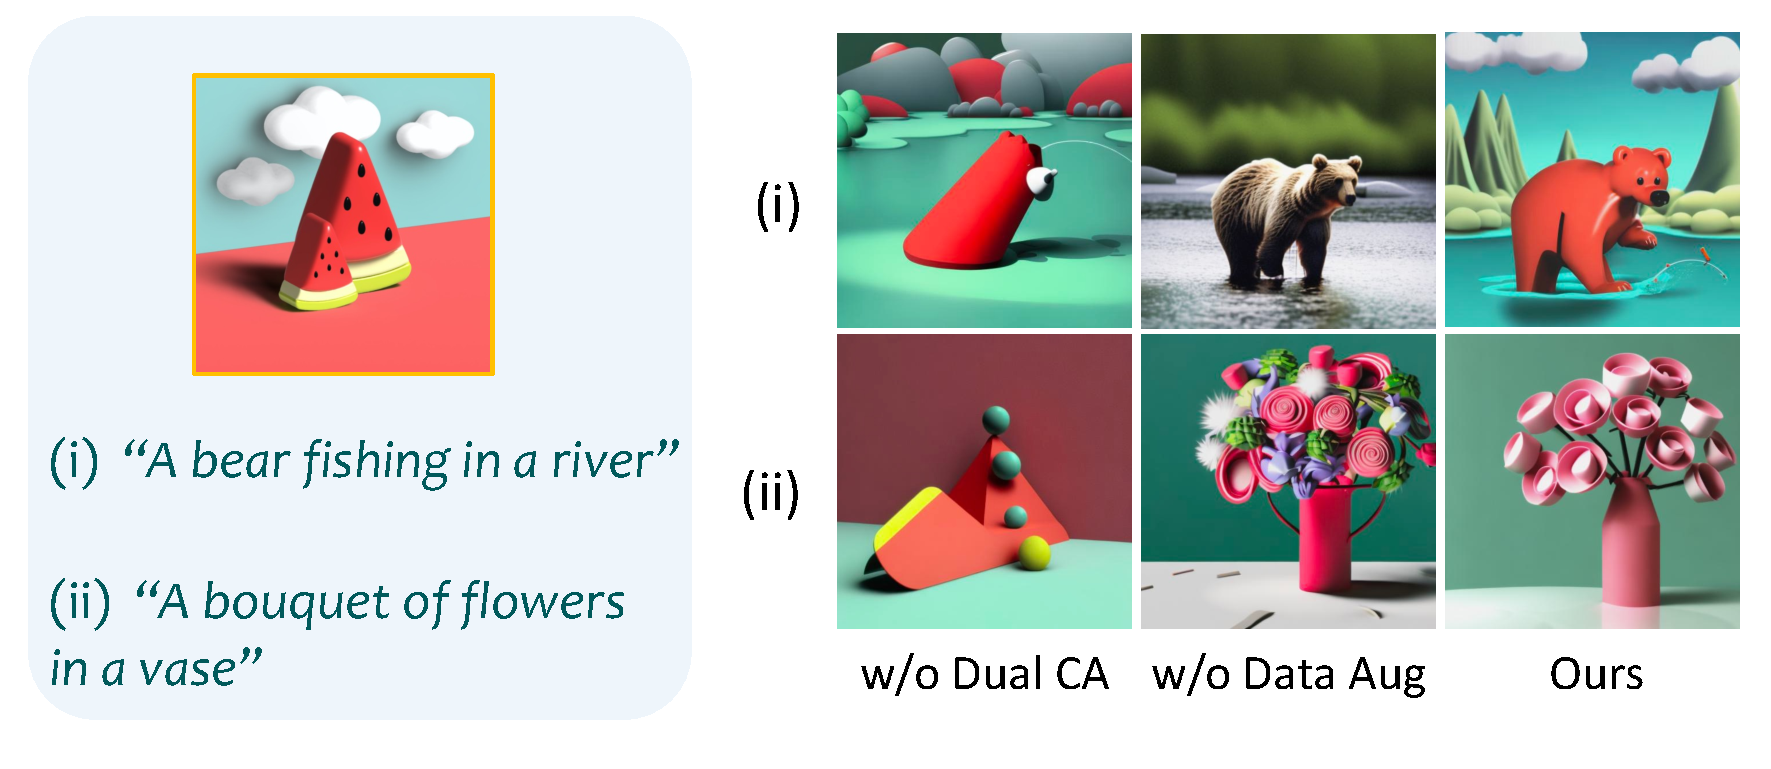
\includegraphics[width=\linewidth]{figures/ablation_img_1.pdf}
    \vspace{-3em}
    \caption{Effects of dual cross-attention and data augmentation.} 
    \label{fig:ablation_img_1_2}
    \vspace{-1em}
\end{figure}


\vspace{-0.5em}
\paragraph{Multi-Reference based Guidance.}
AnimateDiff~\cite{guo2023animatediff} denotes a paradigm to turn personalized SD (i.e., SD fine-tuned on specific-domain images via LoRA~\cite{hu2022lora} or Dreambooth~\cite{dreambooth}) for video generation, namely combined with pre-trained temporal blocks of T2V models. It can generate very impressive results if the personalized SD is carefully prepared, however, we find it struggle to achieve as satisfactory results if only a handful of style reference images are available for training.
We conduct an evaluation on 60 text-style pairs with multi-references, as presented in Sec.~\ref{sec:test_dataset}. We train Dreambooth~\cite{dreambooth} models for each style and incorporate them into AnimateDiff based on their released codebase. Thanks to the flexibility of Q-Former, our method also supports multiple reference images in a tuning-free fashion, i.e. computing the image embeddings of each reference image and concatenating all embeddings as input to the Q-Former.
Results are compared in Table~\ref{tab:video_quan_multi_ref} and Figure~\ref{fig:result_multi_ref} respectively.

According to the results, AnimateDiff struggles to achieve high-fidelity stylistic appearance while tends to generate close-to-realism results despite the style references are typical artistic styles. In addition, it is vulnerable to temporal artifacts. As the trained personalized-SD can generate decent stylistic images (provided in the supplementary materials), we conjecture that the performance degradation is caused by the incompatibility from the pre-trained temporal blocks and independently trained personalized-SD models, which not only interrupts temporal consistency but also weakens the stylistic effect.
In contrast, our method can generate temporal consistent videos with high style conformity to the reference images and accurate content alignment with the text prompts. Furthermore, using multiple references can further promote the performance, which offers additional advantages in practical applications.


%---------------------------------
\subsection{Ablation Study}
\label{subsec:ablation}
%---------------------------------

\begin{figure}[!t]
    \centering
    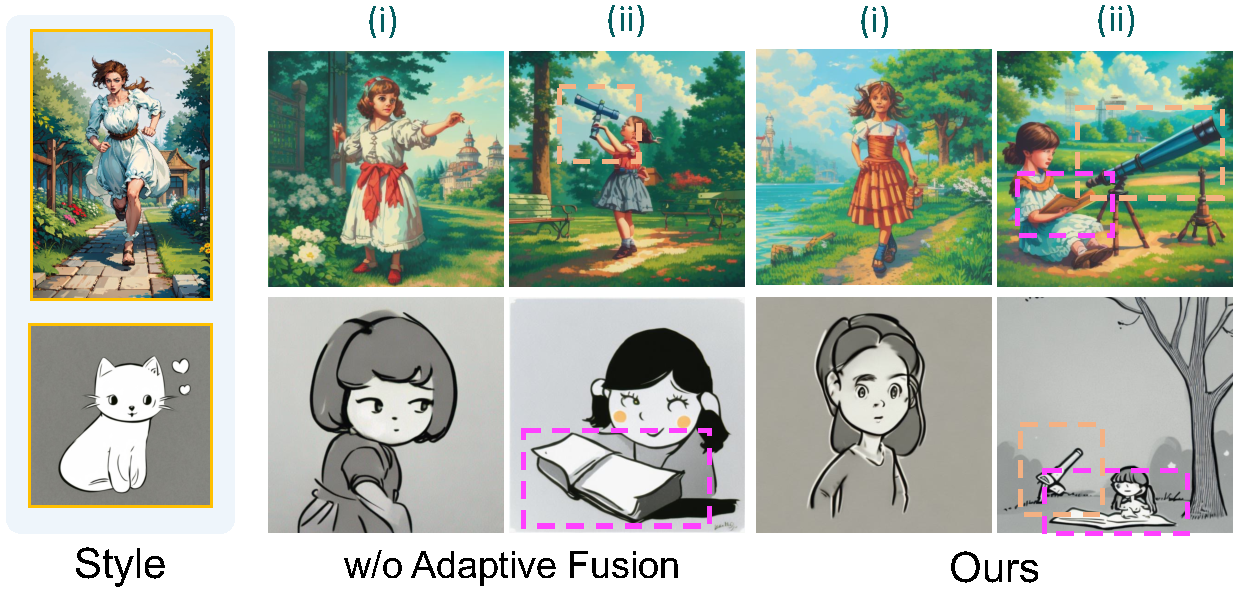
\includegraphics[width=\linewidth]{figures/ablation_no_scale.pdf
    }
    \vspace{-2em}
    \caption{Effect of adaptive content-style fusion. It shows superiority in generalization to extreme cases, e.g. long text description. Two text prompts are used: (i) A little girl; (ii) \textit{A little girl \textcolor[RGB]{255, 64, 255}{reading a book} in the park, with \textcolor[RGB]{244, 177, 131}{a telescope} nearby pointed at the sky}.}
    \label{fig:ablation_no_fusion}
    \vspace{-0.7em}
\end{figure}

% We make ablation studies on some important designs of our method, including data augmentation, module architectures, and training strategies, to validate their effectiveness.

\paragraph{Data Augmentation.}
We first study the effectiveness of content-style decoupled data augmentation. As depicted in Table~\ref{tab:ablation_img}, training with the original image-caption pairs restricts the model's ability to extract style representations, leading to lower style conformity. For example, as shown in Figure~\ref{fig:ablation_img_1_2}, method without data augmentation fails to capture the "3D render" style from the reference.


\paragraph{Dual Cross-Attention.} 
As discussed in Sec.~\ref{subsec:style_modulation},  we make a comparison between \textit{attach-to-text} and \textbf{dual cross-attention} to study their effects. Results are presented in Table ~\ref{tab:ablation_img} and Figure~\ref{fig:ablation_img_1_2}, revealing that \textit{attach-to-text} tends to directly fuse the content from the reference image and the text prompts rather than combining the text-based content and image-based style. This indicates the effectiveness of \textbf{dual cross-attention} in facilitating content-style decoupling.


\paragraph{Adaptive Style-Content Fusion.}
As previously discussed in Figure~\ref{fig:scale_factor_viz}, our proposed adaptive style-content fusion module demonstrates effectiveness in adaptively processing various conditional contexts. It benefits the generalization ability of model to deal with diverse combinations of content prompt and style image. Figure~\ref{fig:ablation_no_fusion} reveals that although the baseline can handle easy prompt inputs like "A little girl", it struggles to accurately generate all objects described in longer prompts. In contrast, the adaptive fusion module can achieve decent text alignment for long text descriptions thanks to its flexibility to adaptive balance between content and style.

\paragraph{Two-Stage Training Scheme.}
Our proposed training scheme consists of two stages, i.e., style adapter training and temporal adaption. To show its necessity, we build two baselines: (i) \textit{w/o Temporal Adaption}: that we train a style adapter on image data and apply it directly to stylized video generation without finetuning; (ii) \textit{joint training}: that we conduct style adapter training and temporal blocks finetuning on image-video dataset simultaneously.
As depicted in Table~\ref{tab:ablation_video}, baseline (i) exhibits inferior temporal consistency when applied directly to video, and undermines the content alignment and style conformity. As for baseline (ii), the learning of style embedding extraction seems to be interfered by the joint finetuning of temporal blocks, which impedes it to generate desirable stylized videos.


\begin{table}[!t]
\centering

\caption{Ablation studies on style modulation designs. The performance is evaluated based on the style-guided T2I generation.}
\label{tab:ablation_img}
\vspace{-1em}
    
\small
% \renewcommand\arraystretch{1.2}
  \begin{tabular}{ccc} % {@{}lc@{}}
    % \toprule
    \hline
    Methods & \texttt{CLIP-Text} $\uparrow$ & \texttt{CLIP-Style} $\uparrow$ \\
    \hline
    Ours & 0.3028 & 0.4836 \\
    ~w/o Data Augmentation & 0.3173 & 0.4005 \\
    w/o Dual Cross Attention & 0.0983 & 0.7332 \\
    w/o Adaptive Fusion & 0.2807 & 0.4925 \\
    \hline
  \end{tabular}
\vspace{-1em}
\end{table}


\begin{table}[!t]
\centering
\vspace{1em}

\caption{Ablation study on our two-stage training scheme.}
\vspace{-1em}
\label{tab:ablation_video}
% \renewcommand\arraystretch{1.5}
\resizebox{\linewidth}{!}{

\begin{tabular}{c c c cc} % {@{}lc@{}}
    % \toprule
    \toprule
    \multirow{2}{*}{Methods} & \multirow{2}{*}{CLIP-Text $\uparrow$} & \multirow{2}{*}{CLIP-Style $\uparrow$} & \multicolumn{2}{c}{Temporal Consistency} \\
    \cmidrule(lr){4-5}
      & & &
     ~CLIP-Temp $\uparrow$~ & \makecell{W.E.($\times10^{-3}$) $\downarrow$}\\
    \midrule
    w/o Temporal Adaption  & 0.2691 & 0.3923 & 0.9612 & 47.88 \\
    Joint Training & 0.3138 & 0.2226 & 0.9741 & 24.74 \\
    Two-Stage(ours) & \textbf{0.2726} & \textbf{0.4531} & \textbf{0.9892} & \textbf{18.73} \\
    \bottomrule
  \end{tabular}
}

    \vspace{-1em}
  
\end{table}

%
% \begin{figure}[!t]
%     \centering
%     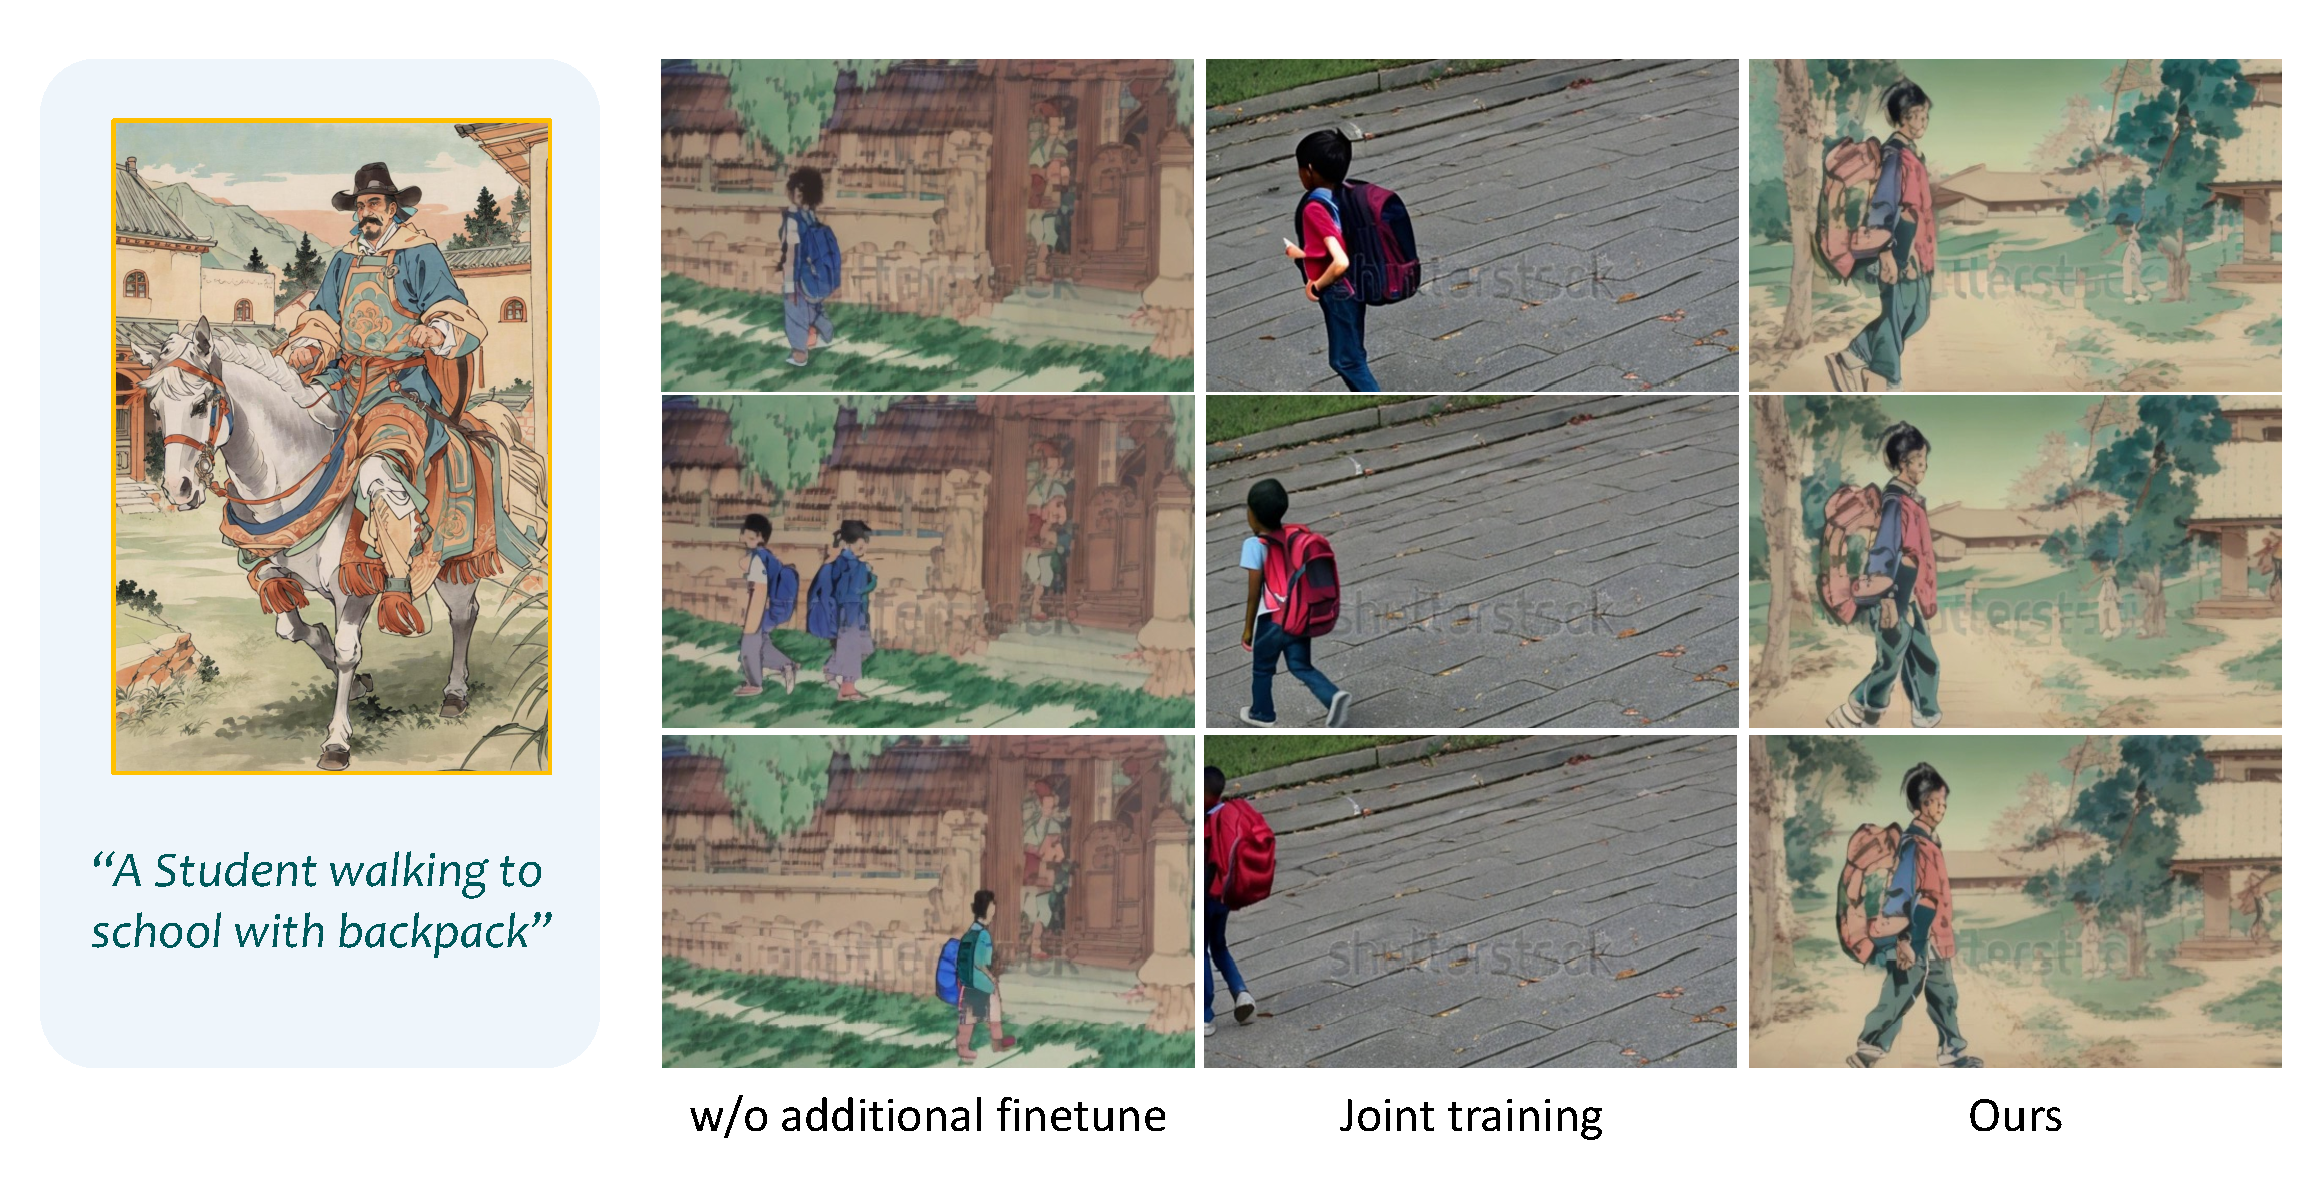
\includegraphics[width=\linewidth]{figures/ablation_two_stage.pdf}
%     \vspace{-2em}
%     \caption{Comparison on the effects of different training schemes.}
%     \label{fig:ablation_two_stage}
%     \vspace{-1em}
% \end{figure}


